\chapter{Fast Pauli Polynomial manipulation}
\label{appendix:FPPM}
Hamiltonian could be decomposed to linear combination of 
several local Hamiltonians.

\begin{equation}
    H = \sum_i \lambda_i H_i
\end{equation}

The common decomposition is using Pauli terms, $H_i = P_{j(i)} = \Pi_{k} \sigma_l(k)^m$.
Since, Pauli terms form an orthonormal basis of the matrix space, 
the decomposition is well-defined on general $n$ qubit Hilbert space with 
Hilbert-Schmidt inner product.

\begin{equation}
    \lambda_i = \langle P_{j(i)} | H \rangle = \frac{1}{2^n} \tr(P_{j(i)} * H)
\end{equation}

The Pauli term representation is called \textit{Pauli-polynimial} of the given Hamiltonian $H$.
However, in large $n$, since the matrix dimension increases with exponential complexity,
the decomposition process requires huge computational resources 
in Hamiltonian analysis and Pauli-polynomial manipulation.

The time complexity of the matrix multiplication is $O(8^n)$, for $n$ qubit Hilbert space.
In addition, it is only about single Pauli term, so that the total coefficient cost is 
$O(32^n)$. It is because that we cannot know what terms are zero in the given 
Hamiltonian and we have to test the all Pauli-terms.

Moreover, constructing the original Hamiltonian with matrix form
from the Pauli polynomial also arises in many situation.
Basic method is constructing each Pauli matrices with tensor products 
of 2-dim Pauli matrices, $\sigma_{i}, i \in \{0, 1, 2, 3\}$ 
and calculating a linear combination of them.
It is called \textit{term-by-term} method.
The complexity of term-by-term method rely on the complexity of 
single $n$-fold Pauli matrix term, $f(n)$,
and the number of non-zero terms in the polynomial, $k$.
Therefore, the complexity of the composition is $O(k(f(n) + 4^n))$.
There are $4^n$ number of Pauli terms, the worst case is $O(16^n + 4^n f(n))$.


\section{Decomposition}

\subsection{Tensorized method}


\subsection{Term-by-Term methods}

\section{Composition}
\subsection{PauliComposer}

\subsection{Inverse of the Tensorized method}

Since, the tensorized method is just a basis transformation, 
the inverse transformation is well defined, 
however, without the coefficient matrix of the Pauli-polynomial 
the inverse algorithm could not be used to construct the original 
Hamiltonian matrix. In the original paper by Hantzko et al \cite{hantzko_tensorized_2023},
they didn't find the way so that only mentioned about the decomposition method.

\begin{equation}
    \label{eq:restore}
    \begin{array}{ccc}
        c_0 &=& \frac{1}{2} (A_{11} + A_{22})\\
        c_1 &=& \frac{1}{2} (A_{12} + A_{21})\\
        c_2 &=& \frac{i}{2} (A_{12} - A_{21})\\
        c_3 &=& \frac{1}{2} (A_{11} - A_{22})\\
    \end{array}
\end{equation}.

In 2024, Kim found a way based on the XZ representation of the 
Paili terms. In addition, he showed that XZ representation is one type of 
coefficient matrix basis.

\begin{theorem}
    For a given simplex representation, $(n_x, n_z)$ of the given Paili term, $P$,
    their index, $(i, j)$, in coefficient matrix is determined as 
    $$(i, j) = (n_z, n_x^\wedge n_z)$$

    where, ${}^\wedge$ is a XOR bitwise operator. 
\end{theorem}

\textbf{Proof} 
From $i$-th iteration of the TPD algorithm of $2^n$ dim square matrix, 
the unit sub-matrix dimension is $2^{n-i}$ and there are 4 block matrices, see Figure \ref{fig:tpd_diagram}.
With Eq(\ref{eq:xz_decompose}), the result matrix of $i-th$ iteration is

\begin{equation}
    \begin{bmatrix}
        \sigma_0 \cdot \sigma_0 & \sigma_1 \cdot \sigma_0\\
        \sigma_1 \cdot \sigma_3 & \sigma_0 \cdot \sigma_3\\
    \end{bmatrix}
    = 
    \begin{bmatrix}
        0_x \cdot 0_z & 1_x \cdot 0_z\\
        1_x \cdot 1_z & 0_x \cdot 1_z\\
    \end{bmatrix}
\end{equation}

where, $0_z, 1_z, 0_x, 1_x$ are XZ binary representation of Pauli term of $i$-th decimal.
For row index, $2^{i} * nz_i, nz_i\in \{0_z, 1_z\}$ the Z-binary determine
the row index movement, if $nz_i = 1_z$, the row location is changed else it is not.
For column index, the column index changed by $+0$ if $(1_x, 0_z)$ or $(0_x, 1_z)$, 
else $+2^{n-i}$ if $(0_x, 0_z)$ or $(1_x, 1_z)$.
It is a simple XOR binary opertor, therby 
$2^{n-i} * nz_i^{\wedge}nx_i, \, nz_i\in \{0_z, 1_z\}, nx_i \in \{0_x, 1_x\}$

Thus, we have (i, j) coefficient index of XZ representation by iteration from 1-th to $n$-th. 

\begin{equation}
    \begin{array}{clcc}
    i =& \sum_{k=0}^{n-1} 2^{k} nz_k &=& nz\\
    j =& \sum_{k=0}^{n-1} 2^{k} nz_k^{\wedge} nx_k &=& nz^{\wedge}nx
    \end{array}
\end{equation}

where $nz_k, nx_k$ are $k$-th binary element of $nz, nx$ binary representation of the given Pauli term $\square$.

The time complexity of the TPD is $O(8^n)$ and it is not different for single term and the 
full term polynomial. 
Comparing to Qiskit, and Pennylane methods we can observe the efficient of the 
routine in the worst case.

\begin{figure}
    \centering
    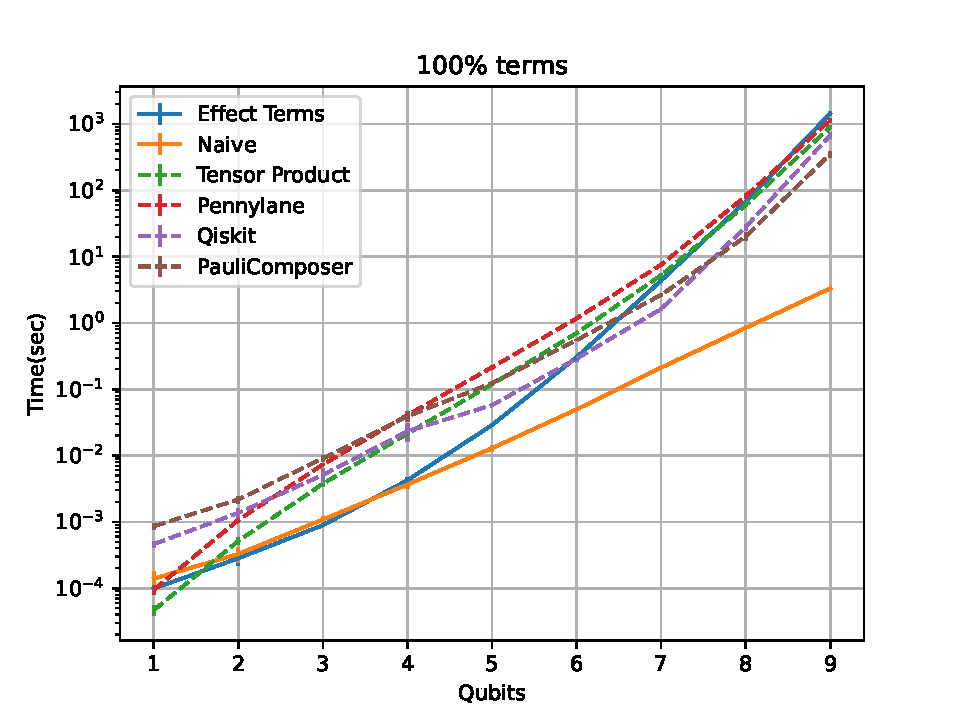
\includegraphics[width=0.7\textwidth]{media/1_terms.pdf}
    \caption{Benchmarks for matrix composition of Puali polynomials with the algorithm 1, 2 with Qiskit, Pennylane,
    PauliComposer, and standard tensor product methods, for $n = 1$ to $n = 9$. The percentages of the each case represents
    how many coefficients are non-empty in $4^n$ number of spaces.}
    \label{fig:composition_benchmark}
\end{figure}